\documentclass[a4paper]{article}

%use the english line for english reports
%usepackage[english]{babel}
\usepackage[portuguese]{babel}
\usepackage[utf8]{inputenc}
\usepackage{indentfirst}
\usepackage{graphicx}
\usepackage{verbatim}


\begin{document}

\setlength{\textwidth}{16cm}
\setlength{\textheight}{22cm}

\title{\Huge\textbf{Trench}\linebreak\linebreak\linebreak
\Large\textbf{Relatório Intercalar}\linebreak\linebreak
\linebreak\linebreak

\includegraphics[scale=0.1]{feup-logo.png}\linebreak\linebreak
\linebreak\linebreak
\Large{Mestrado Integrado em Engenharia Informática e Computação} \linebreak\linebreak
\Large{Programação em Lógica}\linebreak
}

\author{\textbf{Grupo xx:}\\
Kevin Amorim - 201207231 \\
Luís Magalhães - 201207224 \\
\linebreak\linebreak \\
 \\ Faculdade de Engenharia da Universidade do Porto \\ Rua Roberto Frias, s\/n, 4200-465 Porto, Portugal \linebreak\linebreak\linebreak
\linebreak\linebreak\vspace{1cm}}

\maketitle
\thispagestyle{empty}

%************************************************************************************************
%************************************************************************************************

\newpage

%Todas as figuras devem ser referidas no texto. %\ref{fig:codigoFigura}
%
%%Exemplo de código para inserção de figuras
%%\begin{figure}[h!]
%%\begin{center}
%%escolher entre uma das seguintes três linhas:
%%\includegraphics[height=20cm,width=15cm]{path relativo da imagem}
%%\includegraphics[scale=0.5]{path relativo da imagem}
%%\includegraphics{path relativo da imagem}
%%\caption{legenda da figura}
%%\label{fig:codigoFigura}
%%\end{center}
%%\end{figure}
%
%
%\textit{Para escrever em itálico}
%\textbf{Para escrever em negrito}
%Para escrever em letra normal
%``Para escrever texto entre aspas''
%
%Para fazer parágrafo, deixar uma linha em branco.
%
%Como fazer bullet points:
%\begin{itemize}
	%\item Item1
	%\item Item2
%\end{itemize}
%
%Como enumerar itens:
%\begin{enumerate}
	%\item Item 1
	%\item Item 2
%\end{enumerate}
%
%\begin{quote}``Isto é uma citação''\end{quote}


%%%%%%%%%%%%%%%%%%%%%%%%%%
\section{O Jogo TRENCH}

\begin{figure}[h!]
\begin{center}
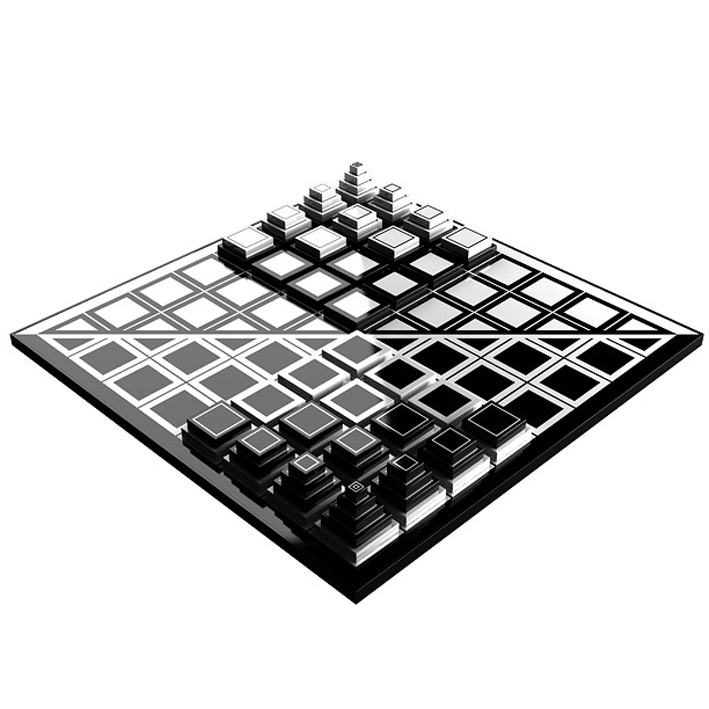
\includegraphics[scale=0.3]{img/game-cover.jpg}
\label{fig:0}
\end{center}
\end{figure}

Trench é um jogo de tabuleiro criado em Portugal por Rui Alípio Monteiro, em 2013. Este é um jogo para 2 jogadores baseado na guerra de trincheiras da 1ª Guerra Mundial. 

Os algoritmos aplicados no jogos seguem os princípios referidos no livro "The Art of the War", de Sun Tzu. A disposição das peças do jogo em losango é inspirada na formação em diamante, originária no exército romano.

\subsection{Objetivo do Jogo}

O objetivo do jogo é capturar todas as peças inimigas. No entanto, nem sempre é possível que tal aconteça (pelas limitações das peças e do tabuleiro), pelo que a vitória ou a derrota regem-se por um sistema de pontuação, explicado em baixo.

\subsection{Início do Jogo}

O jogador que possuir as peças de cor preta inicia o jogo. Cada jogador tem direito a uma jogada por turn. O jogo termina ao fim de 25 jogadas se nenhuma peça for capturada nesse intervalo.

\newpage

\subsection{Tabuleiro de Jogo}

O tabuleiro representa o campo de batalha, com as respetivas trincheiras.
O tabuleiro de jogo tem uma forma em diamante, dividido por uma linha diagonal, que representa a linha das trincheiras (Cada metade do tabuleiro tem uma cor predominante: preto para um jogador, branco para o outro).
O tabuleiro é constítuido por 64 casas (8x8), divididas em dois territórios opostos.

\begin{figure}[h!]
\begin{center}
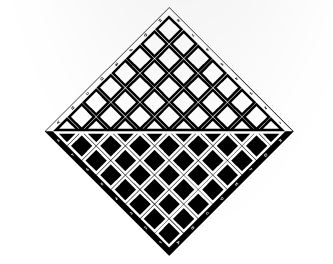
\includegraphics[scale=0.5]{img/board.jpg}
\caption{Tabuleiro de jogo 8x8}
\label{fig:1}
\end{center}
\end{figure}


\subsection{Peças do Jogo}

As peças do jogo são as apresentadas na seguinte tabela:

\begin{figure}[h!]
\begin{center}
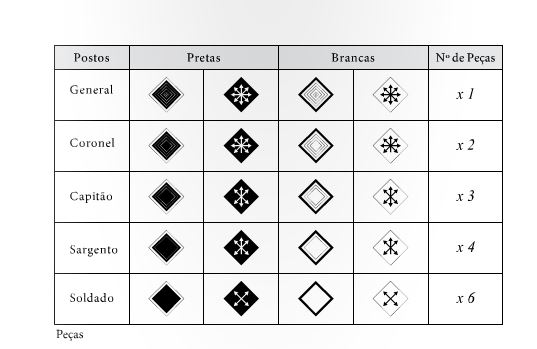
\includegraphics[scale=0.8]{img/pieces.jpg}
\caption{Tabel das peças do jogo}
\label{fig:2}
\end{center}
\end{figure}

 \newpage

Estas possuem uma forma em losango, inspirada nas estrelas usadas pelos soldados em batalha. Estas simbolizam a hierarquia militar em pirâmide.

\begin{figure}[h!]
\begin{center}
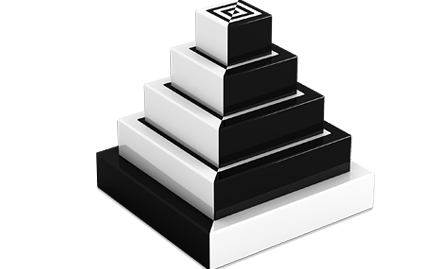
\includegraphics[scale=0.5]{img/piece.png}
\caption{Peça do jogo Trench}
\label{fig:3}
\end{center}
\end{figure}

As peças seguem a seguinte hierarquia (estando no topo o de mais alto nível):

\begin{enumerate}
	\item General
	\item Coronel
	\item Capitão
	\item Sargento
	\item Soldado
\end{enumerate}

\subsubsection{Disposição das Peças}
As peças são dispostas no tabuleiro de forma a simular a formação de um exército Romano, em diamante, como se poder ver na Fig. 5. O general, a peça com maior ranking na hierarquia, fica no topo da metade aliada do tabuleiro, atrás de todo o exército. Na linha da frente ficam os  6 soldados, menor ranking na hierarquia. 

\begin{figure}[h!]
\begin{center}
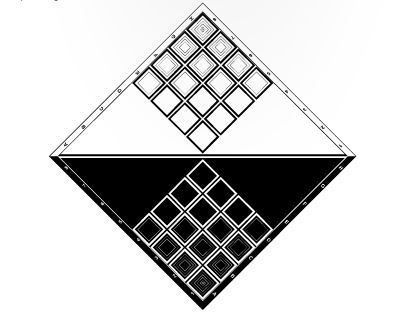
\includegraphics[scale=0.5]{img/pieces-disposition.jpg}
\caption{Disposição das peças do jogo}
\label{fig:4}
\end{center}
\end{figure}

\newpage

\subsubsection{Movimento das Peças}

\begin{itemize}
	\item \textbf{Soldado}: 1 casa (na diagonal em qualquer direção);
	\item \textbf{Sargento}: 2 casas (na diagonal em qualquer direção e para a frente);
	\item \textbf{Capitão}: 3 casas (na diagonal em qualquer direção e tanto para a frente como para trás);'
	\item \textbf{Coronel}: 4 casas (na diagonal em qualquer direção, para frente, esquerda e direita - mas não para trás);
	\item \textbf{General}: 5 casas (em todas as direções);
\end{itemize}

\begin{figure}[h!]
\begin{center}
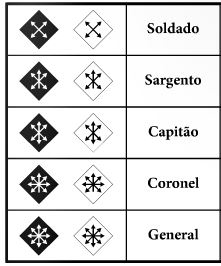
\includegraphics[scale=0.5]{img/pieces-movement.jpg}
\caption{Representação do movimento das peças do jogo}
\label{fig:5}
\end{center}
\end{figure}

\subsubsection{Condições do Movimento das Peças}

\begin{itemize}
	\item O jogador é sempre obrigado a movimentar uma peça, na sua vez.
	\item Nenhuma das peças de jogo pode avançar sobre outra peça (seja do seu ou do exército adversário);
	\item Para capturar uma peça inimiga, a peça do jogador passa a ocupar a parcela quadrada da peça do adversário (terminando o seu movimento imediatamente).
	\item Nenhuma peça é obrigada a percorrer a totalidade das casas que pode percorrer. Isto é, por exemplo, o General pode se mover apenas 1 casa ou 5 casas, conforme o jogador quiser.
\end{itemize}

\newpage

\subsection{A Trincheira}

A trincheira é representada pela linha horizontal no centro do tabuleiro, como referido anteriormente. As peças nesta linha usufruem de um conjunto de vantagens e desvantagens: 


\begin{itemize}
	\item \textbf{1ª Vantagem:} Uma peça na trincheira não pode ser atacada por uma peça adversária. 
	\item \textbf{2ª Vantagem:}Uma peça na trincheira não é obrigada a parar quando ataca uma peça adversária. Portanto, essas podem continuar o seu movimento ou até atacar outras peças, até concluir a sua totalidade de casas a movimentar, ou o jogador decidir parar.

	\item \textbf{1ª Restrição:} Uma peça em trincheira não pode capturar peças adversárias que se encontrem no território aliado (retaguarda). Mas podem ser atacadas por peças adversárias que se encontrem no território aliado. 
	\item \textbf{2ª Restrição:} O Coronel e o General podem se movimentar ao longo de toda a linha da trincheira, mas não podem capturar nenhuma peça adversária que aí se encontre, ficando com os seus movimentos limitados.
\end{itemize}

\newpage

\subsection{Fim do Jogo}

O jogo termina ao fim de duas partidas. Depois de cada partida os jogadores trocam de lado, para que cada um jogue uma vez com as brancas e outra com as pretas. 
	Uma partida termina quando algum jogador capturar todas as peças adversárias. No entanto, se após 50 jogadas ninguém capturar todas as peças adversárias o jogo termina e procede-se a contagem de pontos, segundo a seguinte tabela:

\begin{figure}[h!]
\begin{center}
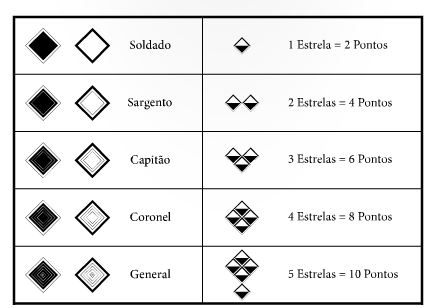
\includegraphics[scale=0.7]{img/points.jpg}
\caption{Valor de cada peça do jogo}
\label{fig:6}
\end{center}
\end{figure}

No final das duas partidas somam-se os pontos feitos por cada jogador em cada partida e ganha o jogo o jogador com mais pontos. Em caso de empate joga-se outra partida e ganha o jogo o jogador que conseguir capturar 40 pontos primeiro. 

\newpage



%%%%%%%%%%%%%%%%%%%%%%%%%%
\section{Representação do Estado do Jogo}

Descrever a forma de representação do estado do tabuleiro (tipicamente uma lista de listas), com exemplificação em Prolog de posições iniciais do jogo, posições intermédias e finais, acompanhadas de imagens ilustrativas.


%%%%%%%%%%%%%%%%%%%%%%%%%%
\section{Visualização do Tabuleiro}

Descrever a forma de visualização do tabuleiro em modo de texto e o(s) predicado(s) Prolog construídos para o efeito.
Deve ser incluída pelo menos uma imagem correspondente ao output produzido pelo predicado de visualização.


%%%%%%%%%%%%%%%%%%%%%%%%%%
\section{Movimentos}

Elencar os movimentos (tipos de jogadas) possíveis e definir os cabeçalhos dos predicados que serão utilizados (ainda não precisam de estar implementados).


\end{document}
